\section{Applications}
\label{sec:app}

There are numerous domains where large scale image processing (LSIP) techniques can be applied. For the scope of this report we are interested in scientific domains where the LSIP can automate tasks performed by the researchers.

\subsection{Animal biometrics}
\label{sec:anim_biom}
In \cite{Kuehl2013}, Kuehl and Burghardt give overview of the methodologies and trends in the emerging field of {\em animal biometrics}. It is an exciting field operating at the intersection between pattern recognition, ecology and information sciences. The subject of the field is to produce computerized systems for phenotypic measurement and interpretation. The main questions for which such systems helps to find the answers to are: how to profile species, individuals and animal behavior by representing phenotypic appearance. Figure \ref{fig:photoIDpen} illustrates the main components of a biometric system. 

\begin{figure}[H]
\begin{center}
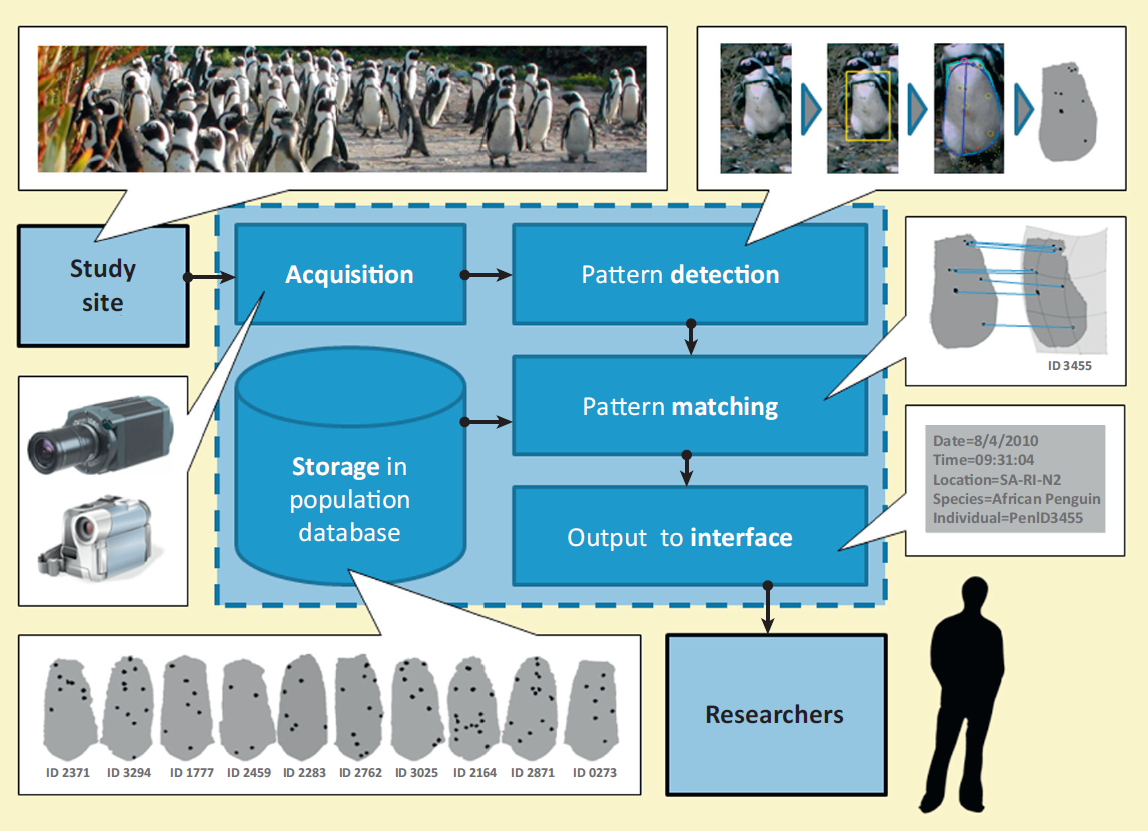
\includegraphics[width=0.68\textwidth]{fig/PhotoIDPenguins}
\end{center}
\caption{Main components of an animal biometric system. This flowchart summarizes how information from a study site is measured and interpreted for the researcher by
an animal biometric system.}
\label{fig:photoIDpen}
\end{figure}
That system parts can either be connected directly on-site or remotely via networks. Each of the components is illustrated, using individual African penguin recognition by spot pattern as an example.  Acquisition: automatic or semi-automatic collection of images or video from fixed field cameras, observers or
the general public. Detection: the use of computer algorithms to search the images to find those that contain the biometric entity of interest and then to extract relevant
information about that entity (e.g., the chest spots of a penguin). Storage: the extracted data on the entity is reduced to a compact mathematical form that can be stored in a
suitable database. Matching: the mathematical data on the entity are then compared with other data already stored in the database to find matches that enable the
individual or the behavior to be identified, using methods akin to the matching of fingerprints to identify humans. Interfacing: presenting the output of the biometric system
to a user or software system for further analysis.

Animal biometrics is important field not only for ecological researchers, but for the general public. For example, in \cite{Kumar2014}, a biometric system for face recognition of pet animals (mainly dogs) have been developed.